\documentclass[border=5pt]{standalone}
\usepackage{pgfplots}
\pgfplotsset{compat=1.18}
\usepackage[T1]{fontenc}
\usepackage{helvet}
\renewcommand{\familydefault}{\sfdefault}

\definecolor{ingestcolor}{HTML}{2196F3}
\definecolor{cpucolor}{HTML}{E65100}
\definecolor{slocolor}{HTML}{2E7D32}
\definecolor{migcolor}{HTML}{7B1FA2}
\definecolor{spikezone}{HTML}{FFF3E0}

\begin{document}
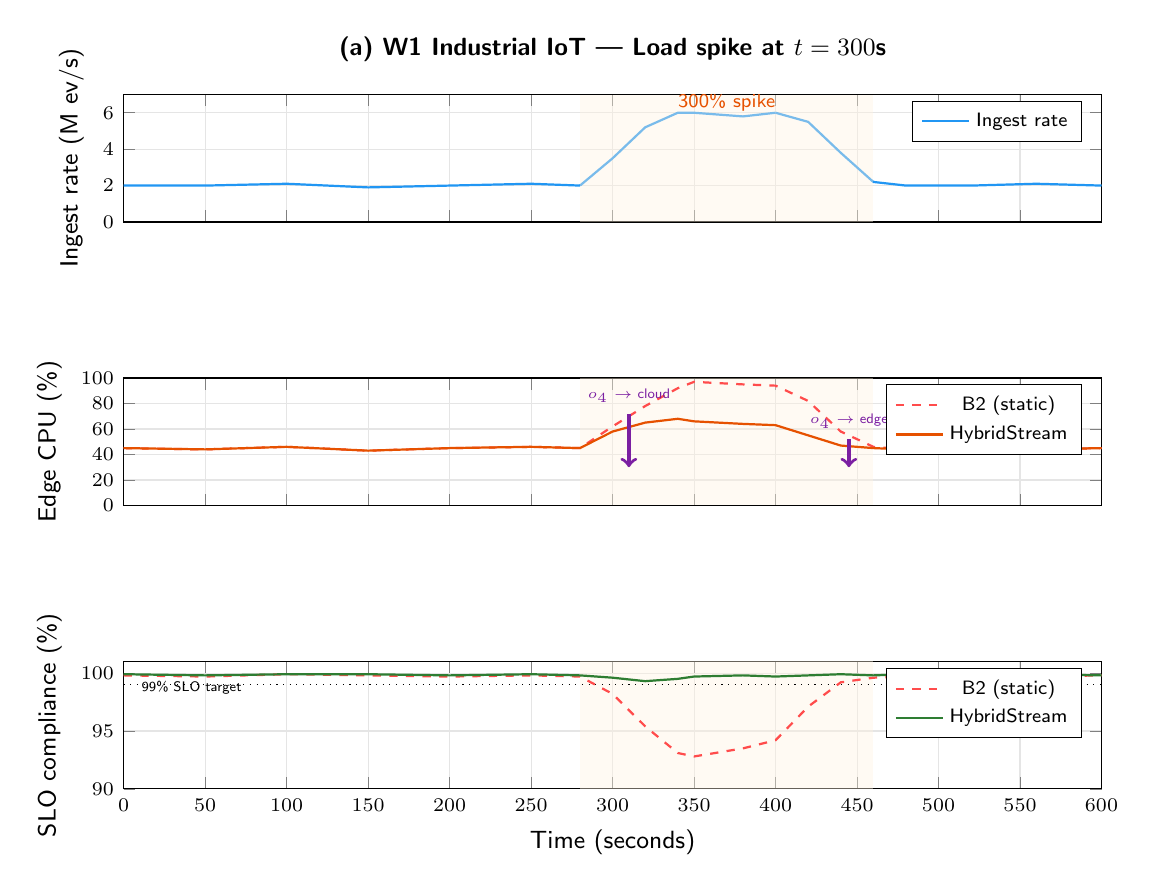
\begin{tikzpicture}
\pgfplotsset{
    every axis/.style={
        width=14cm,
        height=3.2cm,
        xmin=0, xmax=600,
        xlabel style={font=\small},
        ylabel style={font=\small},
        tick label style={font=\scriptsize},
        legend style={font=\scriptsize, at={(0.98,0.95)}, anchor=north east},
        grid=major,
        grid style={gray!20},
    }
}

% Panel (a): Ingest rate
\begin{axis}[
    at={(0,7.2cm)},
    ylabel={Ingest rate (M ev/s)},
    ymin=0, ymax=7,
    xticklabels={},
    title={\small\textbf{(a) W1 Industrial IoT --- Load spike at $t=300$s}},
    title style={at={(0.5,1.05)}},
]
% Baseline period
\addplot[ingestcolor, thick, mark=none] coordinates {
    (0,2.0) (50,2.0) (100,2.1) (150,1.9) (200,2.0) (250,2.1) (280,2.0)
};
% Spike ramp up
\addplot[ingestcolor, thick, mark=none] coordinates {
    (280,2.0) (300,3.5) (320,5.2) (340,6.0) (350,6.0) (380,5.8) (400,6.0)
};
% Spike plateau and ramp down
\addplot[ingestcolor, thick, mark=none] coordinates {
    (400,6.0) (420,5.5) (440,3.8) (460,2.2) (480,2.0) (520,2.0) (560,2.1) (600,2.0)
};
% Spike zone shading
\draw[fill=spikezone, draw=none, opacity=0.4] (axis cs:280,0) rectangle (axis cs:460,7);
\node[font=\scriptsize, text=cpucolor] at (axis cs:370,6.6) {300\% spike};
\legend{Ingest rate}
\end{axis}

% Panel (b): Edge CPU utilization
\begin{axis}[
    at={(0,3.6cm)},
    ylabel={Edge CPU (\%)},
    ymin=0, ymax=100,
    xticklabels={},
]
\draw[fill=spikezone, draw=none, opacity=0.4] (axis cs:280,0) rectangle (axis cs:460,100);
% B2 static
\addplot[red!70, thick, dashed, mark=none] coordinates {
    (0,45) (50,44) (100,46) (150,43) (200,45) (250,46) (280,45)
    (300,62) (320,78) (340,92) (350,97) (380,95) (400,94)
    (420,82) (440,58) (460,46) (480,44) (520,45) (560,44) (600,45)
};
% HybridStream
\addplot[cpucolor, thick, mark=none] coordinates {
    (0,45) (50,44) (100,46) (150,43) (200,45) (250,46) (280,45)
    (300,58) (320,65) (340,68) (350,66) (380,64) (400,63)
    (420,55) (440,47) (460,45) (480,44) (520,45) (560,44) (600,45)
};
% Migration events
\draw[migcolor, very thick, ->] (axis cs:310,72) -- (axis cs:310,30);
\node[font=\tiny, text=migcolor, anchor=south] at (axis cs:310,73) {$o_4 \to$ cloud};
\draw[migcolor, very thick, ->] (axis cs:445,52) -- (axis cs:445,30);
\node[font=\tiny, text=migcolor, anchor=south] at (axis cs:445,53) {$o_4 \to$ edge};
\legend{B2 (static), HybridStream}
\end{axis}

% Panel (c): SLO compliance
\begin{axis}[
    at={(0,0cm)},
    ylabel={SLO compliance (\%)},
    xlabel={Time (seconds)},
    ymin=90, ymax=101,
]
\draw[fill=spikezone, draw=none, opacity=0.4] (axis cs:280,90) rectangle (axis cs:460,101);
% B2 static — drops during spike
\addplot[red!70, thick, dashed, mark=none] coordinates {
    (0,99.8) (50,99.7) (100,99.9) (150,99.8) (200,99.7) (250,99.8) (280,99.7)
    (300,98.2) (320,95.4) (340,93.1) (350,92.8) (380,93.5) (400,94.2)
    (420,97.1) (440,99.2) (460,99.6) (480,99.7) (520,99.8) (560,99.7) (600,99.8)
};
% HybridStream — maintains compliance
\addplot[slocolor, thick, mark=none] coordinates {
    (0,99.9) (50,99.8) (100,99.9) (150,99.9) (200,99.8) (250,99.9) (280,99.8)
    (300,99.6) (320,99.3) (340,99.5) (350,99.7) (380,99.8) (400,99.7)
    (420,99.8) (440,99.9) (460,99.8) (480,99.9) (520,99.8) (560,99.9) (600,99.8)
};
% SLO threshold
\addplot[black, thin, dotted, mark=none] coordinates {(0,99) (600,99)};
\node[font=\tiny, anchor=west] at (axis cs:5,98.7) {99\% SLO target};
\legend{B2 (static), HybridStream}
\end{axis}

\end{tikzpicture}
\end{document}
